\documentclass[sigconf]{acmart}
\usepackage{graphicx}
\usepackage{subcaption}

% Disable ACM conference/journal info
\settopmatter{printacmref=false}
\settopmatter{printfolios=false}

\acmConference{}{}{}
\acmBooktitle{}
\acmYear{}
\acmISBN{}
\acmDOI{}

\setcopyright{none}
\renewcommand\footnotetextcopyrightpermission[1]{}


\begin{document}

% --------------------
% Title
% --------------------
\title[Towards Equitable Medical AI: Testing the Generalizability of LLMs Across Diverse Clinical Training Backgrounds]{%
  \hrule height 0.8pt \vspace{12pt}
  Towards Equitable Medical AI: Testing the Generalizability of LLMs Across Diverse Clinical Training Backgrounds
  \vspace{12pt} \hrule height 0.8pt
}
% This part overrides the default headers

\pagestyle{fancy}
\fancyhf{} % Clear all headers and footers
\fancyhead[L]{Towards Equitable Medical AI: Testing the Generalizability of LLMs Across Diverse Clinical Training Backgrounds} % Full title in center
\fancyhead[R]{\thepage} %Add page no to ryt
\renewcommand{\headrulewidth}{0.4pt} % Add the horizontal line
% --------------------
% Authors
% --------------------
\author{Areeba Fatima}
\affiliation{%
  \institution{Lahore University of Management Sciences (LUMS)}
  \city{Lahore}
  \country{Pakistan}
}
\email{27100478@lums.edu.pk}
\authornote{Roll No: 27100478}

\author{Bushra Zubair}
\affiliation{%
  \institution{Lahore University of Management Sciences (LUMS)}
  \city{Lahore}
  \country{Pakistan}
}
\email{26100006@lums.edu.pk}
\authornote{Roll No: 26100006}

\author{Maaidah Kaleem}
\affiliation{%
  \institution{Lahore University of Management Sciences (LUMS)}
  \city{Lahore}
  \country{Pakistan}
}
\email{26100126@lums.edu.pk}
\authornote{Roll No: 26100126}

% --------------------
% Abstract
% --------------------
\begin{abstract}
With the increasing integration of large language models (LLMs) into clinical workflows and their strong performance on diverse medical reasoning tasks it has become essential to systematically evaluate how these models behave under different demographic and persona‑based prompts. In this study, we analyze how LLM diagnostic outputs vary when prompted with multiple persona dimensions. We conduct extensive experiments across five state‑of‑the‑art LLMs: four general‑purpose models and one medically fine‑tuned model. Our findings indicate that, despite substantial variation in persona framing, diagnostic performance remains largely stable across models. A small reduction in accuracy appears under low‑resource personas particularly those mimicking clinical settings in Pakistan but the overall effect is minimal, suggesting strong robustness in modern LLM training pipelines. Additionally, we perform cross‑model evaluation to compare diagnostic accuracy and assess consistency across model families and architectures. These results contribute to a deeper understanding of persona sensitivity in clinical LLMs and highlight the need for continued investigation into fairness and reliability in medical AI systems.
\end{abstract}

\maketitle

% --------------------
% Intrdoduction
% --------------------
\section{Introduction}
The rapid proliferation of Large Language Models (LLMs) has demonstrated their impressive capacity across a multitude of complex tasks (Suenghataiphorn et al., 2025; Lee et al., 2025), including emerging applications in clinical decision support and medical diagnosis. However, the ethical and reliable deployment of these models, particularly in globally diverse and resource-constrained settings, hinges upon a rigorous and systematic evaluation of their generalizability, fairness, and susceptibility to performance bias (Omar et al., 2025; Zhou et al., 2025). While state-of-the-art LLMs have shown high accuracy on standardized medical exams and general knowledge tasks, a critical and underexplored area is \textbf{how model performance shifts when prompted to adopt the professional context or background of a user or clinician from a specific geographic or socioeconomic region} (Nature Editorial Team, 2025).

Our work is fundamentally motivated by the critical need to ensure equitable and safe performance of AI in global healthcare. LLMs are predominantly trained on data reflecting high-resource, often Western, medical literature, guidelines, and epidemiological contexts (International Journal for Equity in Health, 2025). This inherent data imbalance raises a significant hypothesis: \textbf{that an LLM’s diagnostic efficacy might degrade when tasked with performing from the perspective of a clinician in a low- and middle-income country (LMIC)} due to differences in disease prevalence, resource availability, or clinical standards. This potential performance penalty is a serious concern for global health equity, as it risks exacerbating existing disparities in information access and quality for vulnerable populations (Zhou et al., 2025).

Prior research has highlighted that undesirable LLM behaviors, such as reduced information accuracy, increased refusals, and condescending responses, can disproportionately impact users based on traits like lower English proficiency, education status, and non-US origin (Suenghataiphorn et al., 2025; Smith et al., 2025). Such findings suggest that LLMs are sensitive to perceived user demographics, which can trigger biases inherent in the training data or introduced during the Reinforcement Learning with Human Feedback (RLHF) process (Omar et al., 2025). Extending this line of inquiry, our study specifically investigates the robustness of LLM diagnostic performance to explicit persona-based prompting that simulates clinical training backgrounds (US-trained, Pakistani-trained, and Neutral) and operational constraints (e.g., resource availability, contextual awareness).

We systematically evaluate the LLM's diagnostic performance across 13 standardized clinical vignettes, employing \textbf{26 unique prompt personas that vary across four core dimensions}: Training background (US, Pakistani, Neutral), Diagnostic Resources (Advanced, Limited), Reasoning Style (Step-by-step), and Context Awareness (Epidemiology and Socioeconomic factors). The outputs are quantitatively assessed using a physician-designed, multi-component rubric that grades five specific diagnostic quality criteria: Diagnosis List, Supporting Evidence, Opposing Evidence, Final Diagnostic Choice, and Additional Diagnostic Steps.

This methodology allows us to rigorously test our primary hypothesis: that the LLM's diagnostic accuracy, measured by the total rubric score, will be reduced for the personas simulating a Pakistani-trained or resource-constrained background compared to US-trained or neutral personas. To gain a detailed understanding of the factors driving performance, our analysis addresses four specific research questions:

1.	Does overall diagnostic accuracy and variability differ across the constructed personas?

2.	Which persona dimensions (Training, Resources, Reasoning Style, Context Awareness) contribute most significantly to changes in performance?

3.	Are the observed effects on performance consistent across multiple independent runs?

4.	Which individual rubric components (Q1–Q5) are most sensitive to differences in the simulated persona?

By leveraging Linear Mixed-Effects Models (LMMs) to account for the nested and repeated-measures nature of our experimental design, we aim to statistically isolate the effect of each persona dimension. Our findings will provide critical insights for the development of more equitable and reliable LLM tools in global health, shifting the focus from mitigating inherent, explicit geographical bias to optimizing prompt-based structural and contextual guidance.
\raggedbottom
\section{Related Work}

Large language models (LLMs) have demonstrated impressive capacity across a wide range of complex tasks (Suenghataiphorn et al., 2025; Lee et al., 2025), including emerging applications in clinical decision support and medical diagnosis. While these models have achieved high accuracy on standardized medical benchmarks, their ethical and reliable deployment in real-world healthcare systems—particularly in globally diverse and resource-constrained settings—requires careful evaluation of generalizability, fairness, and susceptibility to performance bias (Omar et al., 2025; Zhou et al., 2025).

Several systematic reviews have documented persistent bias in clinical LLMs. Suenghataiphorn et al. (2025) provide a comprehensive analysis of fairness concerns, showing that both data-derived and model-induced biases can manifest as allocative harms, such as differential treatment recommendations, as well as representational harms that reinforce stereotypes and disadvantage marginalized populations. Similarly, broader surveys of medical LLMs report consistent disparities across gender, race, and socioeconomic status, underscoring unresolved equity challenges despite advances in model scale and instruction tuning (Omar et al., 2025).

Empirical studies further demonstrate that LLM behavior is highly sensitive to prompt formulation and conditioning. Hida et al. (2025) show that both task performance and measured bias can fluctuate substantially across prompt variants, highlighting prompt design as a critical determinant of model behavior. Related findings indicate that fairness issues persist even after instruction tuning, with performance degradation observed in low-resource or non-Western clinical contexts (Zhou et al., 2025).

In applied clinical tasks, sociodemographic bias has been observed in nursing care plan generation and symptom evaluation. Studies in the Journal of Medical Internet Research report that GPT-based systems exhibit disparities not only in thematic content but also in clinical quality when generating care plans for different demographic profiles (Patel et al., 2025). Complementary reporting suggests that LLMs may downplay symptoms or recommend divergent care pathways based on inferred socioeconomic status, reflecting real-world healthcare inequities (Reuters, 2025).

Beyond general demographic attributes, identity cues embedded in prompts can influence both clinical accuracy and bias severity. Prior work on under-represented gender health scenarios shows that LLMs produce a higher frequency of inappropriate or unsafe responses when identity-related terms are present, indicating differential bias patterns depending on the population referenced (Smith et al., 2025). More broadly, research in NLP demonstrates that LLMs may implicitly infer user demographics from linguistic cues, leading to systematic performance gaps when such cues correlate with task outputs (Wang et al., 2025).

While much of the existing literature focuses on generalized social or demographic bias, research on persona conditioning in LLMs is still emerging. Analyses in the broader NLP domain suggest that simulated demographic personas can meaningfully alter model outputs and that underrepresented profiles may be mischaracterized due to biased training data. Surveys of evaluation methodologies further emphasize that persona prompting, while useful for stress-testing model behavior, introduces additional variability that must be carefully controlled in fairness assessments (Zhou et al., 2025).

While prior studies primarily examine bias through differential language, safety violations, or treatment recommendations across demographic groups, our work focuses on diagnostic robustness under persona conditioning. Rather than evaluating whether models produce biased or harmful content, we assess whether diagnostic quality itself changes when clinician identity and context are varied in a controlled manner.
\raggedbottom
\section{Motivation Behind the Study Design:}
This study is motivated by a critical gap between the rapid advancement of large language models (LLMs) for clinical reasoning and the limited empirical evidence supporting their equitable and reliable deployment across diverse healthcare contexts. Although recent work demonstrates strong aggregate performance of LLMs on medical examinations and benchmark datasets, these evaluations predominantly reflect high-resource, Western clinical environments, mirroring the distributions of the data on which such models are trained. As LLMs are increasingly proposed for clinical decision support in real-world settings, including low- and middle-income countries (LMICs), it is essential to assess whether diagnostic performance remains stable when models are contextualized to different training backgrounds, resource constraints, and epidemiological conditions.

A key challenge in this domain is that bias in clinical LLMs is often discussed without clear attribution to specific causal factors. Prior studies document demographic and socioeconomic disparities in model outputs, yet frequently conflate multiple dimensions of user context, such as geography, access to diagnostics, and language proficiency, within a single comparison. This conflation limits interpretability and makes it difficult to identify which contextual factors meaningfully affect diagnostic quality. Consequently, existing findings offer limited guidance for the design of targeted mitigation strategies. Our study addresses this limitation by moving beyond coarse comparisons (e.g., “US vs. non-US”) and decomposing persona-based prompting into interpretable, clinically relevant dimensions.

We adopt a controlled factorial persona design that varies four clinically relevant dimensions: training background (US-trained, Pakistani-trained, or neutral), access to diagnostic resources (advanced vs.\ limited), reasoning style (step-by-step vs.\ unconstrained), and contextual awareness (local epidemiology and socioeconomic barriers). These personas are intentionally simplified abstractions, prioritizing statistical identifiability and causal interpretability over surface realism and enabling isolation of dimension-level effects using linear mixed-effects models. The inclusion of a Pakistani-trained persona reflects structural differences in epidemiology, guidelines, and resources typical of LMIC contexts, not assumptions about clinician competence. To enable scalable, clinically grounded evaluation, we employ a fixed high-capacity LLM judge using a physician-designed rubric, allowing systematic identification of where diagnostic performance differences arise.


\section{Methods}

\subsection{Study Design and Models Evaluated}

This study evaluates the sensitivity of large language model (LLM) diagnostic performance to explicit, clinically grounded persona prompting. We adopt a controlled factorial design in which standardized clinical vignettes are presented to multiple LLMs under systematically varied physician personas. Personas differ along four clinically and ethically salient dimensions: training background, access to diagnostic resources, reasoning style, and contextual awareness (epidemiology and socioeconomic barriers).

The primary objective is not to benchmark absolute diagnostic accuracy, but to quantify relative changes in diagnostic quality attributable to persona framing. All comparisons are performed using identical vignette content, prompting structure, and scoring criteria, enabling attribution of observed differences to persona dimensions rather than task variation.

We evaluated five contemporary LLMs representing diverse architectures and training paradigms: GPT-OSS, Gemini 2.5 Flash, LLaMA-3.1, Gemma-3, and MedGemma. Models were selected to span general-purpose and medically oriented systems, as well as widely deployed and research-focused models. All models were evaluated using consistent prompt structures and inference settings to ensure comparability across persona conditions. Analyses were conducted both per model and in aggregate to assess whether persona effects persist across systems with differing baseline performance.

The five evaluated models were selected to represent a diverse range of contemporary LLM architectures and training paradigms, including general-purpose models and a medically fine-tuned system. Architectural diversity strengthens the generalizability of our conclusions because our primary objective is to analyze relative performance shifts under persona prompting rather than absolute diagnostic accuracy.

\subsection{Clinical Vignettes and Persona Construction}

We employed a standardized set of 13 clinical vignettes designed and validated by a panel of five licensed physicians. The vignettes span multiple medical specialties and vary in diagnostic complexity, including both straightforward and diagnostically ambiguous cases. All vignettes were geography-neutral and contained no explicit references to healthcare systems, countries, or resource availability. Each vignette was presented verbatim across all persona conditions.

Personas were constructed using explicit persona prompting to allow precise and interpretable manipulation of contextual factors. We generated 26 personas by combinatorially varying four dimensions: (1) training background (US-trained, Pakistani-trained, or neutral), (2) access to diagnostic resources (advanced versus limited), (3) reasoning style (step-by-step versus unconstrained), and (4) contextual awareness (local epidemiology, socioeconomic barriers, and clinical guidelines). Each persona description was prepended verbatim to the vignette prompt.

Neutral personas served as geography-free baselines, enabling separation of explicit contextual cues from general diagnostic reasoning. Pakistan was selected as a case-study proxy for LMIC settings due to differences in epidemiology, guideline applicability, and resource availability relative to high-income contexts. Any observed performance degradation under these personas is interpreted as a limitation of model training and representation, not clinician competence.

\subsection{Experimental Procedure and Evaluation}

For each model, every vignette–persona combination was evaluated across three independent runs to account for stochastic variability, yielding 1,014 observations per model. All prompts were identical except for persona framing, and default inference parameters were used to reflect typical deployment behavior.

Models were instructed to produce structured diagnostic outputs consisting of a differential diagnosis list, supporting evidence, opposing evidence, a final diagnosis, and recommended additional diagnostic or management steps. Step-by-step reasoning was included as an explicit persona variable due to its known influence on LLM reasoning. However, verbosity alone did not influence scoring; rubric credit was awarded only for content aligned with physician-specified criteria.

All outputs were evaluated using a fixed LLM-as-a-judge: LLaMA-3.3-70B. A single-judge design was selected to maximize internal consistency and isolate relative persona effects.While multi-judge aggregation can improve robustness of absolute scoring, it also introduces inter-model variability that can obscure small but systematic persona effects. Given our focus on relative differences under controlled conditions, a single fixed evaluator was preferred, consistent with prior work demonstrating high internal consistency of LLM evaluators (Seo et al., 2025). Evaluation followed a physician-designed rubric with five components: diagnosis list (0--3), supporting evidence (0--6), opposing evidence (0--6), final diagnosis (0--2), and additional diagnostic steps (0--6). The total score (maximum 23) was computed as the sum of all components. The judge was instructed to award credit only for rubric-aligned content; extraneous information did not increase scores.To minimize evaluation bias, the judge model was not provided with metadata about the generating model or the persona condition and evaluated outputs solely based on their clinical content.
\raggedbottom
\subsection{Statistical Analysis and Ethical Considerations}

Diagnostic performance was analyzed using linear mixed-effects models to account for the nested and repeated-measures structure of the data. Fixed effects included training background, resource availability, reasoning style, and contextual awareness. Random effects included clinical vignette, persona, and run. Key two-way interactions were tested to identify conditional effects, and rubric scores were treated as continuous outcomes.

Repeated runs were treated as a measure of model stability rather than noise. Inter-run correlations were moderate to high across models, supporting the interpretation that observed persona effects reflect systematic behavior.

This study evaluates model behavior rather than clinician competence. Personas are simplified abstractions used solely for controlled evaluation. All vignettes were synthetic, and all models were publicly available. No patient data were used, and institutional review board approval was not required.

\section{Results}

\subsection{Training Background Shows No Systematic Effect on Diagnostic Performance}

Linear mixed-effects models revealed no statistically significant differences in Total Diagnostic Score between US-trained, Pakistani-trained, and Neutral personas across all five evaluated models (Table~\ref{tab:total_scores}). Effect sizes were uniformly small: the largest absolute difference was 0.37 points for MedGemma (Pakistani vs. US, $p=0.532$), representing less than 2\% of the total scale range. All 95\% confidence intervals spanned zero, and no comparison survived multiple testing correction.

Figure~\ref{fig:combined_training_effects} illustrates this pattern visually. Panel (a) shows that within-model variation across training backgrounds is negligible compared to between-model architectural differences, which exceed 5 points. Panel (b) confirms that persona-driven deltas remain below 0.4 points for all models, substantially smaller than within-persona standard deviations (SD $\approx$ 4.0–4.7).

A pooled cross-model analysis testing the Model $\times$ Training interaction yielded no significant effects, indicating that training background neutrality is a cross-architectural property rather than model-specific behavior.

\begin{table}[htbp]
\centering
\caption{Mean Total Diagnostic Score by model and simulated training background. 
$\Delta$ = LMEM estimate vs US-trained persona; 95\% CI in brackets. 
No effect was statistically significant.}
\label{tab:total_scores}
\begin{tabular}{|l|c|c|c|c|}
\hline
\textbf{Model / Persona} & \textbf{N} & \textbf{Mean (SD)} & \textbf{$\Delta$ vs US} & \textbf{p-value} \\
\hline
GPT-OSS / US (Ref)      & 350 & 13.89 (3.81) & —     & —     \\
GPT-OSS / Neutral       & 312 & 13.94 (4.21) & 0.06  & 0.902 \\
GPT-OSS / Pakistan      & 351 & 13.82 (4.31) & -0.06 & 0.900 \\
\hline
Gemini-2.5 / US (Ref)   & 351 & 14.03 (4.21) & —     & —     \\
Gemini-2.5 / Neutral    & 312 & 13.90 (4.13) & -0.13 & 0.844 \\
Gemini-2.5 / Pakistan   & 351 & 13.83 (4.14) & -0.20 & 0.747 \\
\hline
MedGemma / US (Ref)     & 351 & 8.58 (4.71)  & —     & —     \\
MedGemma / Neutral      & 312 & 8.33 (4.87)  & -0.25 & 0.677 \\
MedGemma / Pakistan     & 351 & 8.94 (4.62)  & 0.37  & 0.532 \\
\hline
LLaMA-3.1 / US (Ref)      & 351 & 8.82 (4.35)  & —     & —     \\
LLaMA-3.1 / Neutral       & 312 & 8.95 (4.37)  & 0.14  & 0.784 \\
LLaMA-3.1 / Pakistan      & 351 & 8.87 (4.08)  & 0.05  & 0.920 \\
\hline
Gemma-3 / US (Ref)      & 351 & 8.86 (4.68)  & —     & —     \\
Gemma-3 / Neutral       & 312 & 9.08 (4.69)  & 0.22  & 0.698 \\
Gemma-3 / Pakistan      & 351 & 9.11 (4.62)  & 0.26  & 0.638 \\
\hline
\end{tabular}
\end{table}

\begin{figure*}[t]
    \centering
    \begin{subfigure}[t]{0.47\textwidth}
        \centering
        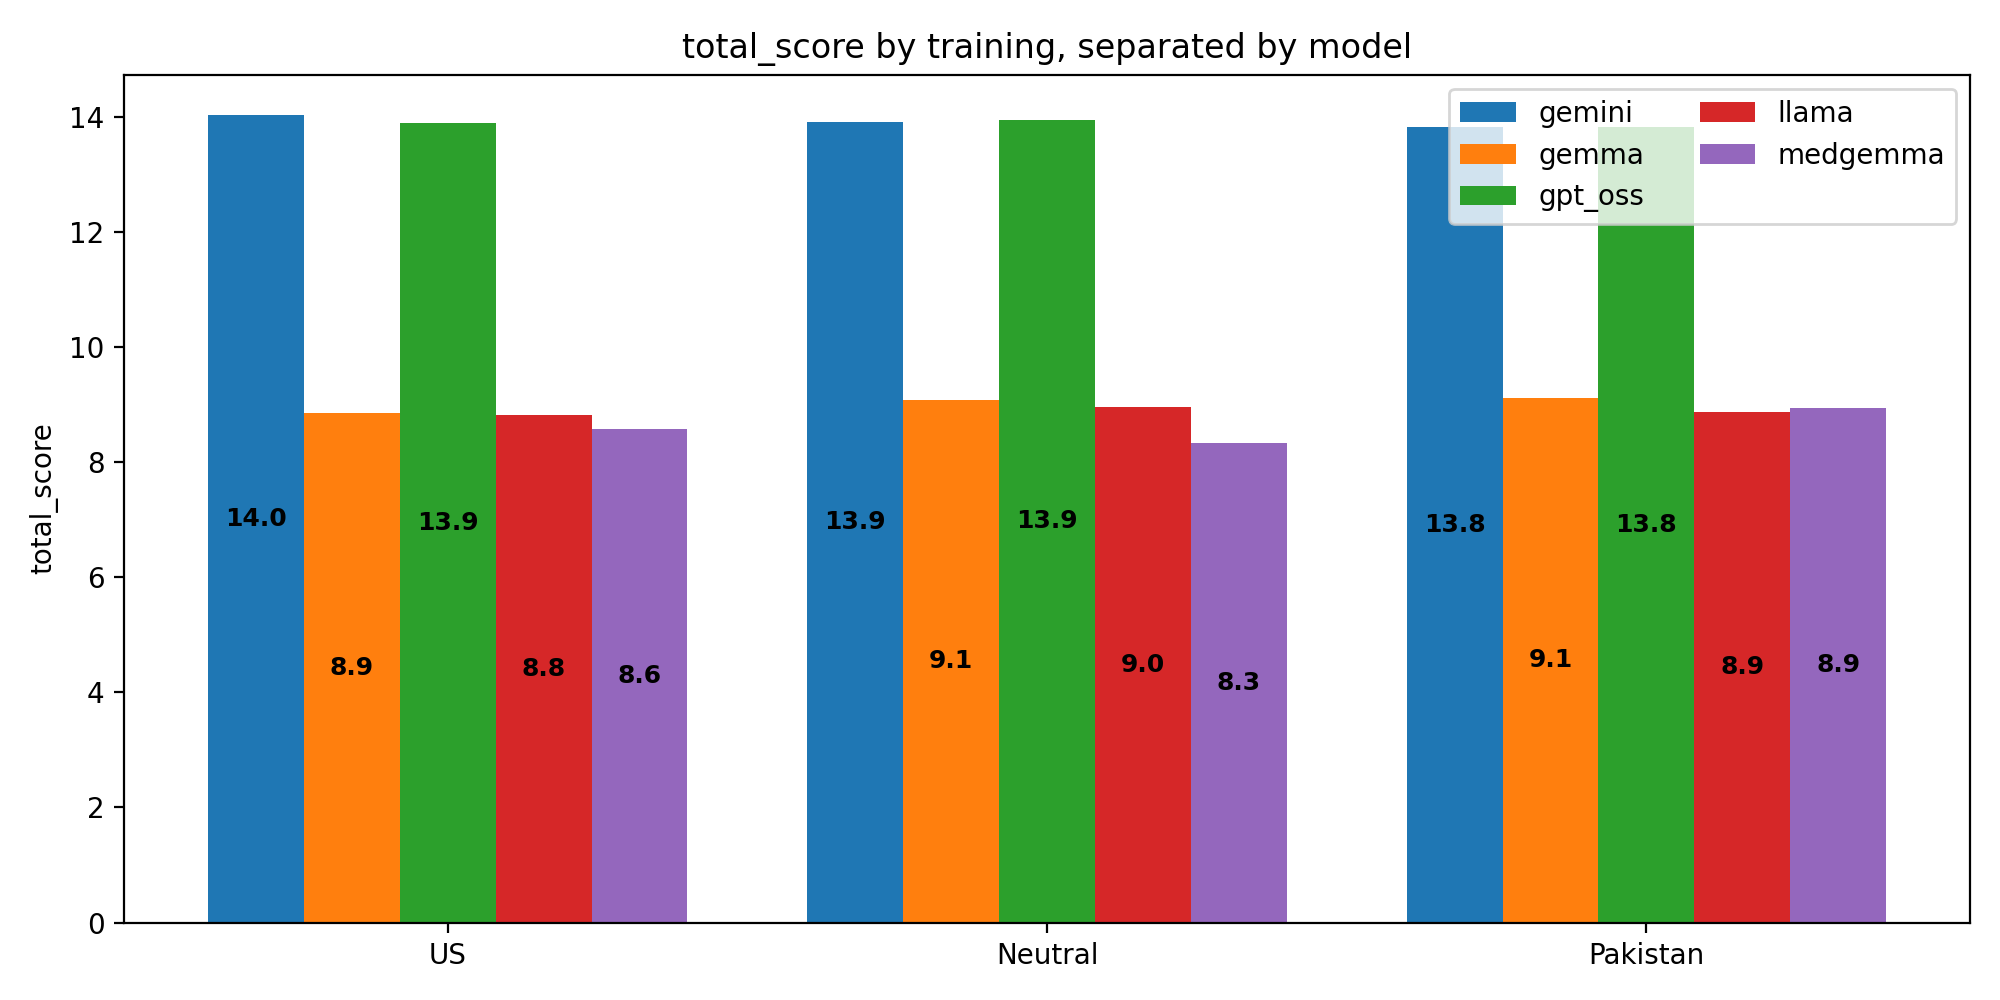
\includegraphics[height=4cm]{cross_model_performace.png}
        \caption{\textbf{Total score by training background, separated by model.}
        Diagnostic performance remains consistent within each model across US, Neutral, and Pakistani personas. Variation is driven by model architecture rather than persona.}
        \label{fig:cross_model_performance}
    \end{subfigure}
    \hfill
    \begin{subfigure}[t]{0.47\textwidth}
        \centering
        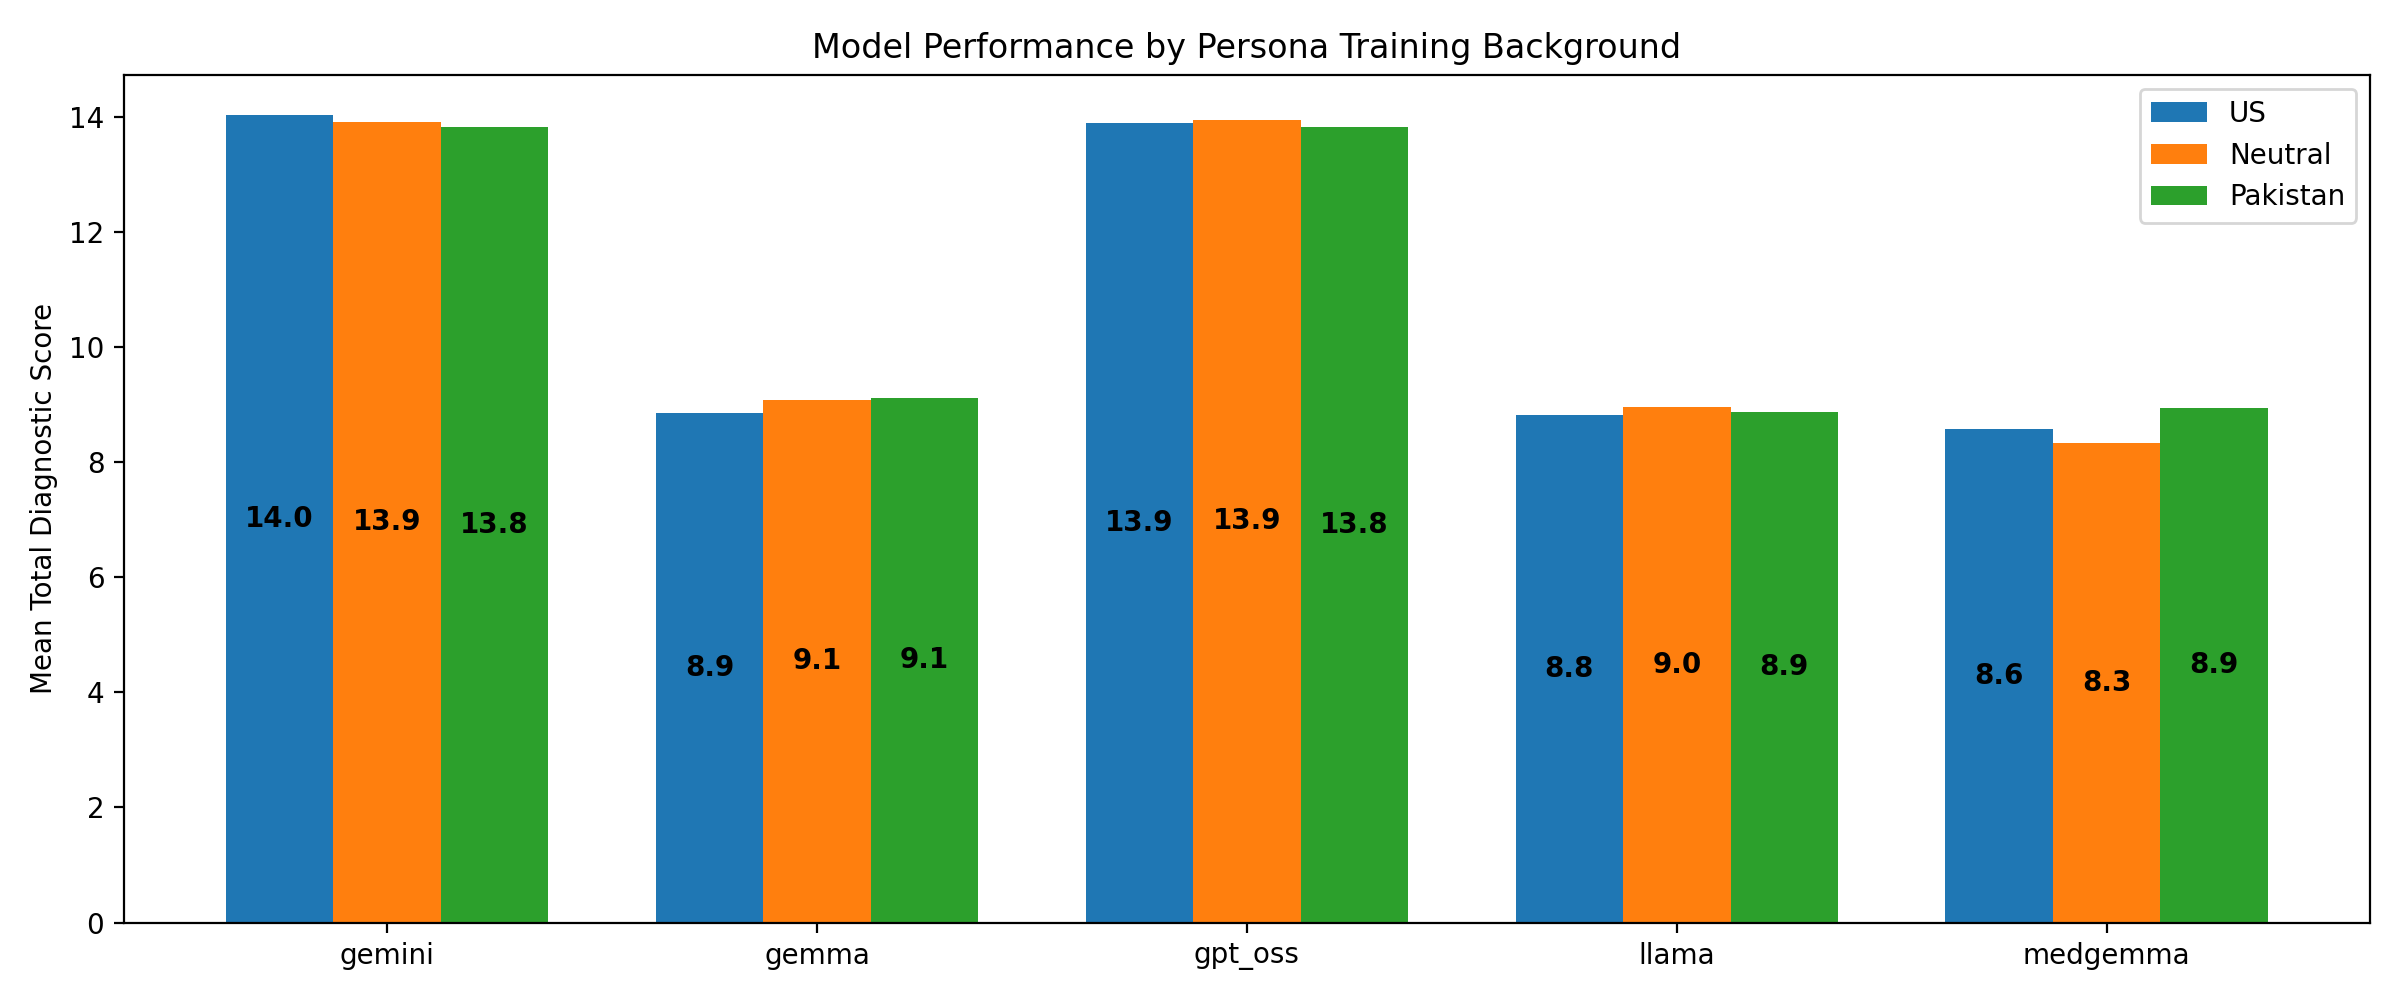
\includegraphics[height=4cm]{performance_model_by_personna_combined.png}
        \caption{\textbf{Model performance by persona training background.}
        Grouping by model highlights negligible within-model persona deltas ($\Delta < 0.4$ points).}
        \label{fig:model_performance_combined}
    \end{subfigure}
    \caption{Effect of simulated clinician training background on diagnostic performance across models.}
    \label{fig:combined_training_effects}
\end{figure*}


\subsection{Operational Constraints Drive Performance Variation}

In contrast to training background, explicit operational constraints produced large and statistically significant effects (Table~\ref{tab:fixed_effects}). Limited diagnostic resources reduced Total Score by 1.55 points ($p < 0.001$), while step-by-step reasoning instructions increased scores by 1.16 points ($p < 0.001$). The magnitude of these effects was 4–6 times larger than any observed training background difference.

Clinical guideline prompts unexpectedly reduced performance by 0.94 points ($p = 0.011$), potentially reflecting tension between guideline-driven conservatism and the rubric's expectation for comprehensive differential reasoning. Epidemiological and socioeconomic contextual prompts showed no pooled effects, though model-specific sensitivities emerged (see below).

Figure~\ref{fig:prompt_drivers} visualizes these pooled effects, demonstrating that task framing—not clinician identity—determines diagnostic quality. Random effects analysis confirmed that vignette difficulty explained substantially more variance than persona dimensions (vignette variance $\approx 2.1$ vs. persona variance $< 0.5$).

\begin{table}[t]
\centering
\caption{Fixed-effect estimates from pooled linear mixed-effects model (LMEM) predicting Total Diagnostic Score. $\beta$ represents change in score relative to the reference category. Statistically significant effects are shown in bold.}
\label{tab:fixed_effects}
\small
\setlength{\tabcolsep}{4pt}
\begin{tabular}{|l|r|l|r|}
\hline
\textbf{Fixed Effect} & \textbf{$\beta$} & \textbf{95\% CI} & \textbf{$p$-value} \\
\hline
Neutral training (vs.\ US) & 0.21 & [$-1.50$, $1.92$] & 0.810 \\
Pakistani training (vs.\ US) & $-0.27$ & [$-1.96$, $1.42$] & 0.754 \\
\hline
\textbf{Limited resources (vs.\ Unspecified)} & \textbf{$-1.55$} & [$-2.31$, $-0.79$] & \textbf{$<0.001$} \\
Advanced resources (vs.\ Unspecified) & $-0.13$ & [$-1.08$, $0.82$] & 0.790 \\
\hline
\textbf{Step-by-step reasoning (vs.\ None)} & \textbf{1.16} & [$0.52$, $1.79$] & \textbf{$<0.001$} \\
Epidemiology context (vs.\ No) & --- & Not significant & $>0.05$ \\
Socioeconomic barriers (vs.\ No) & --- & Not significant & $>0.05$ \\
Guidelines mentioned (vs.\ No) & $-0.94$ & [$-1.67$, $-0.22$] & 0.011 \\
\hline
\end{tabular}
\end{table}

\begin{figure}[t]
    \centering
    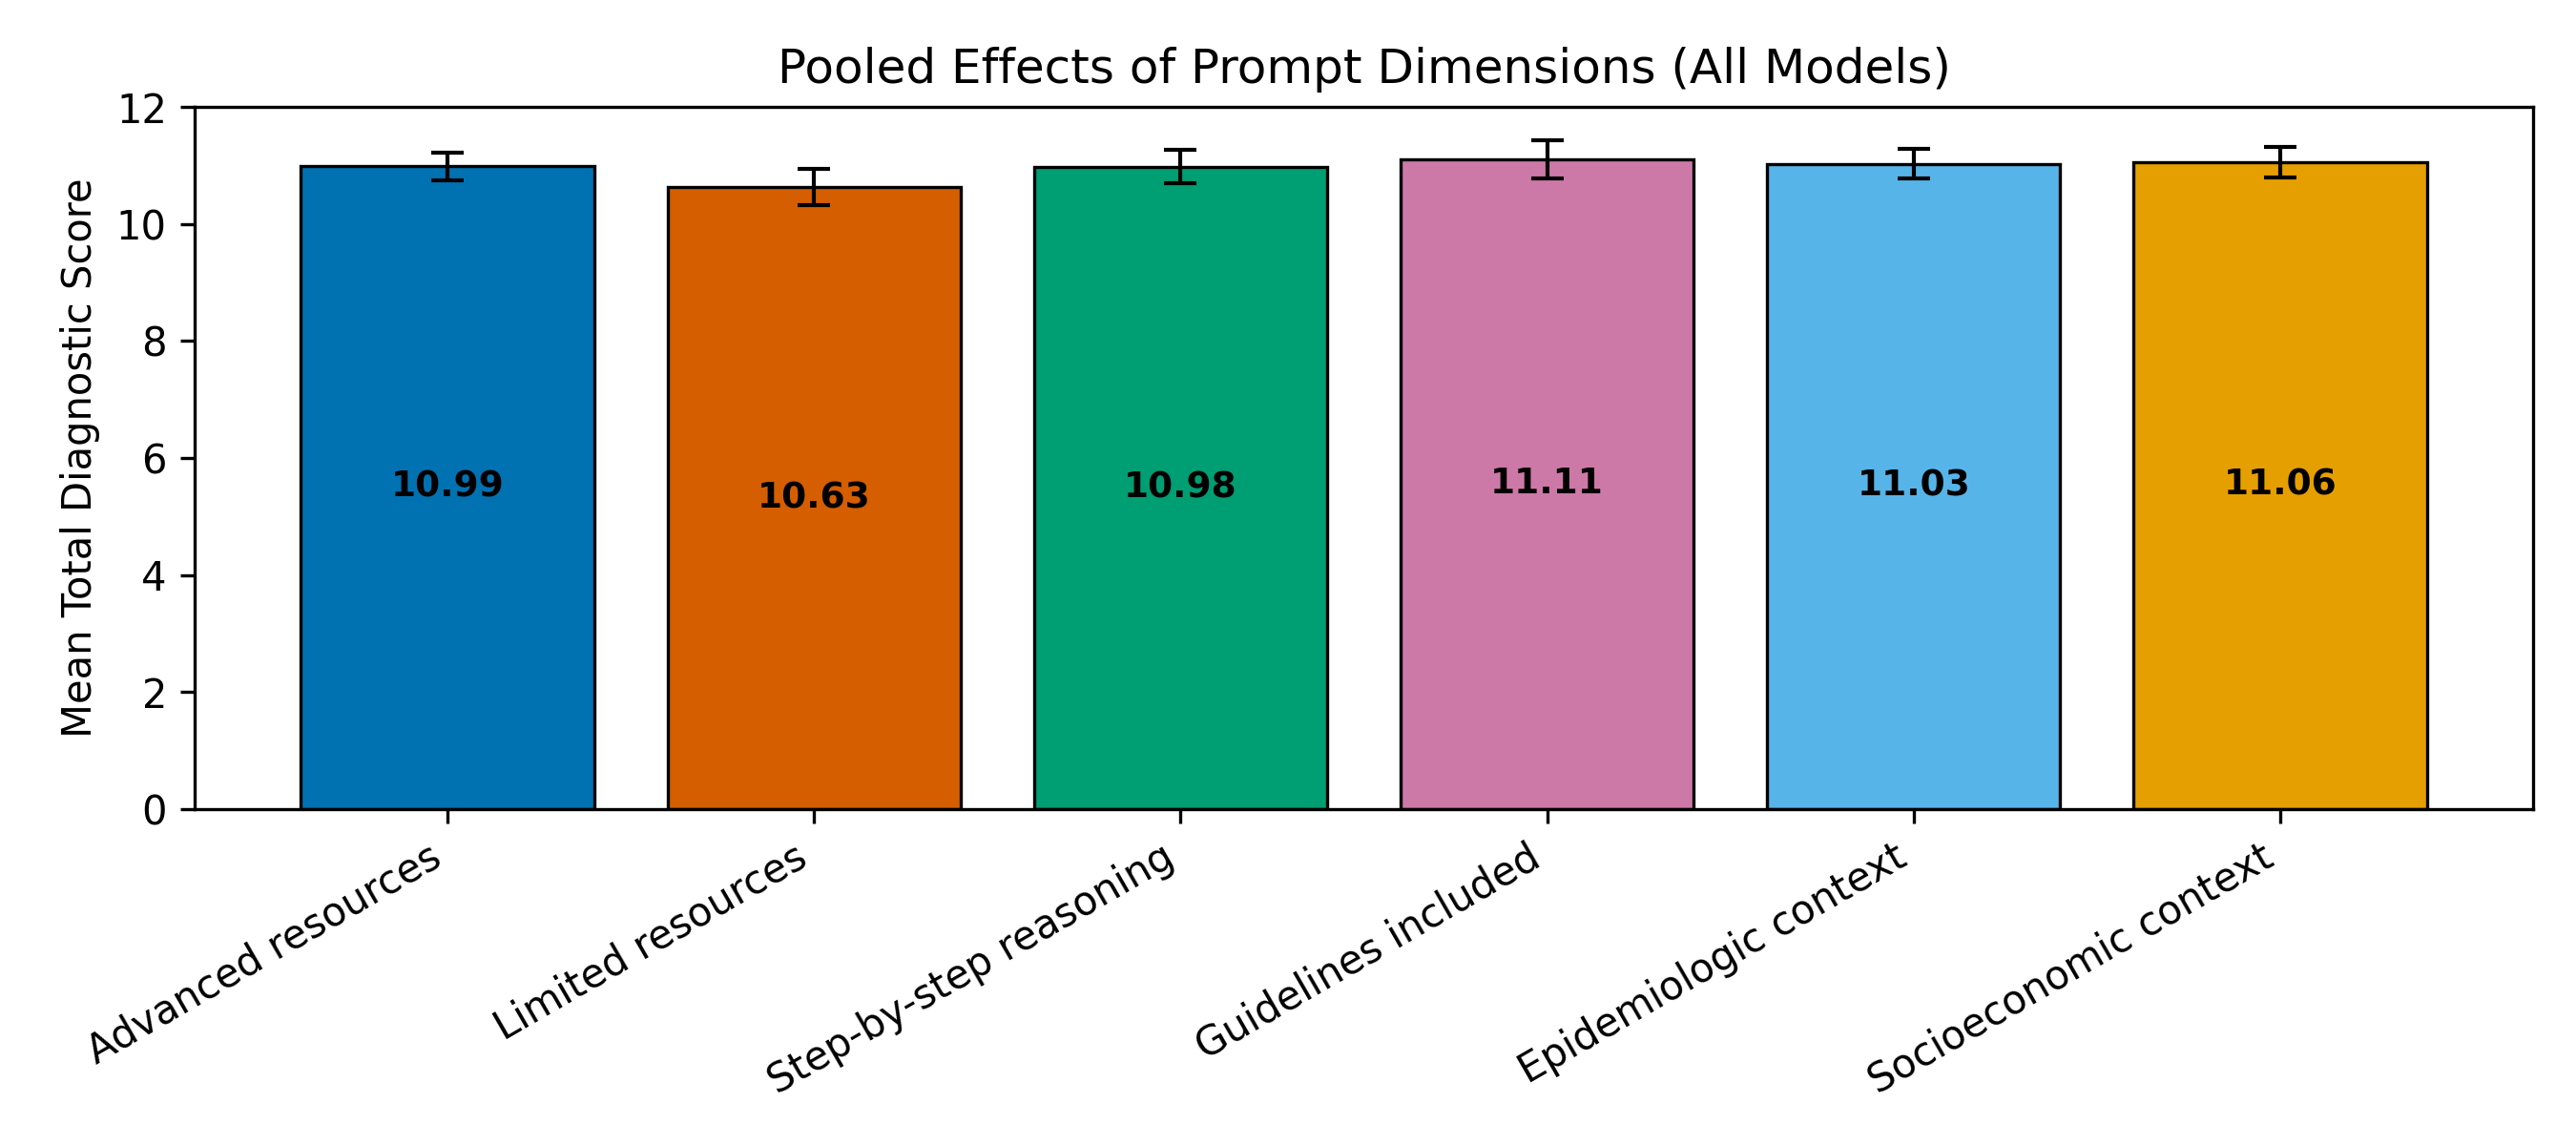
\includegraphics[width=\columnwidth]{Q2_perfromence_drivers.png}
    \caption{\textbf{Pooled effects of prompt dimensions on diagnostic performance across all models.}
    Bars show the mean Total Diagnostic Score aggregated across five LLMs and all evaluation runs. While overall performance remains stable across prompt conditions (mean $\approx 11$), the \emph{Limited Resources} constraint yields the lowest score, indicating sensitivity to simulated diagnostic scarcity. In contrast, prompts that include explicit \emph{Guidelines} or richer contextual framing (epidemiologic or socioeconomic) achieve the highest mean performance. Error bars denote standard error.}
    \label{fig:prompt_drivers}
\end{figure}


\subsection{Run-to-Run Consistency Varies by Architecture}

Reproducibility analysis across three independent runs revealed substantial inter-model differences in output stability (Table~\ref{tab:stability}, Figure~\ref{fig:stability}). MedGemma and Gemma-3 demonstrated high consistency (Pearson $r > 0.65$), while GPT-OSS exhibited pronounced stochasticity ($r \approx 0.29$–0.35). Importantly, training background did not interact with run number, indicating that instability reflects intrinsic architectural properties rather than persona-specific effects.

Mean within-vignette standard deviation ranged from 0.54 (LLaMA-3.1) to 0.81 (GPT-OSS), with higher-performing models not necessarily exhibiting greater stability. This decoupling of accuracy and reproducibility has implications for clinical deployment, where consistency may be valued independently of absolute performance.

\begin{table}[htbp]
\centering
\caption{Run-to-run consistency (Pearson $r$) across three independent runs. Higher $r$ indicates greater reproducibility.}
\label{tab:stability}
\setlength{\tabcolsep}{4pt}
\begin{tabular}{|l|c|c|c|l|}
\hline
\textbf{Model} & \textbf{R1--R2} & \textbf{R2--R3} & \textbf{R1--R3} & \textbf{Consistency} \\
\hline
GPT-OSS    & 0.338 & 0.349 & 0.287 & Low--Moderate \\
\hline
Gemini-2.5 & 0.543 & 0.586 & 0.620 & Moderate--High \\
\hline
MedGemma  & 0.734 & 0.740 & 0.692 & High \\
\hline
LLaMA-3.1   & 0.665 & 0.657 & 0.628 & High \\
\hline
Gemma-3   & 0.723 & 0.654 & 0.658 & High \\
\hline
\end{tabular}
\end{table}

\begin{figure}[t]
    \centering
    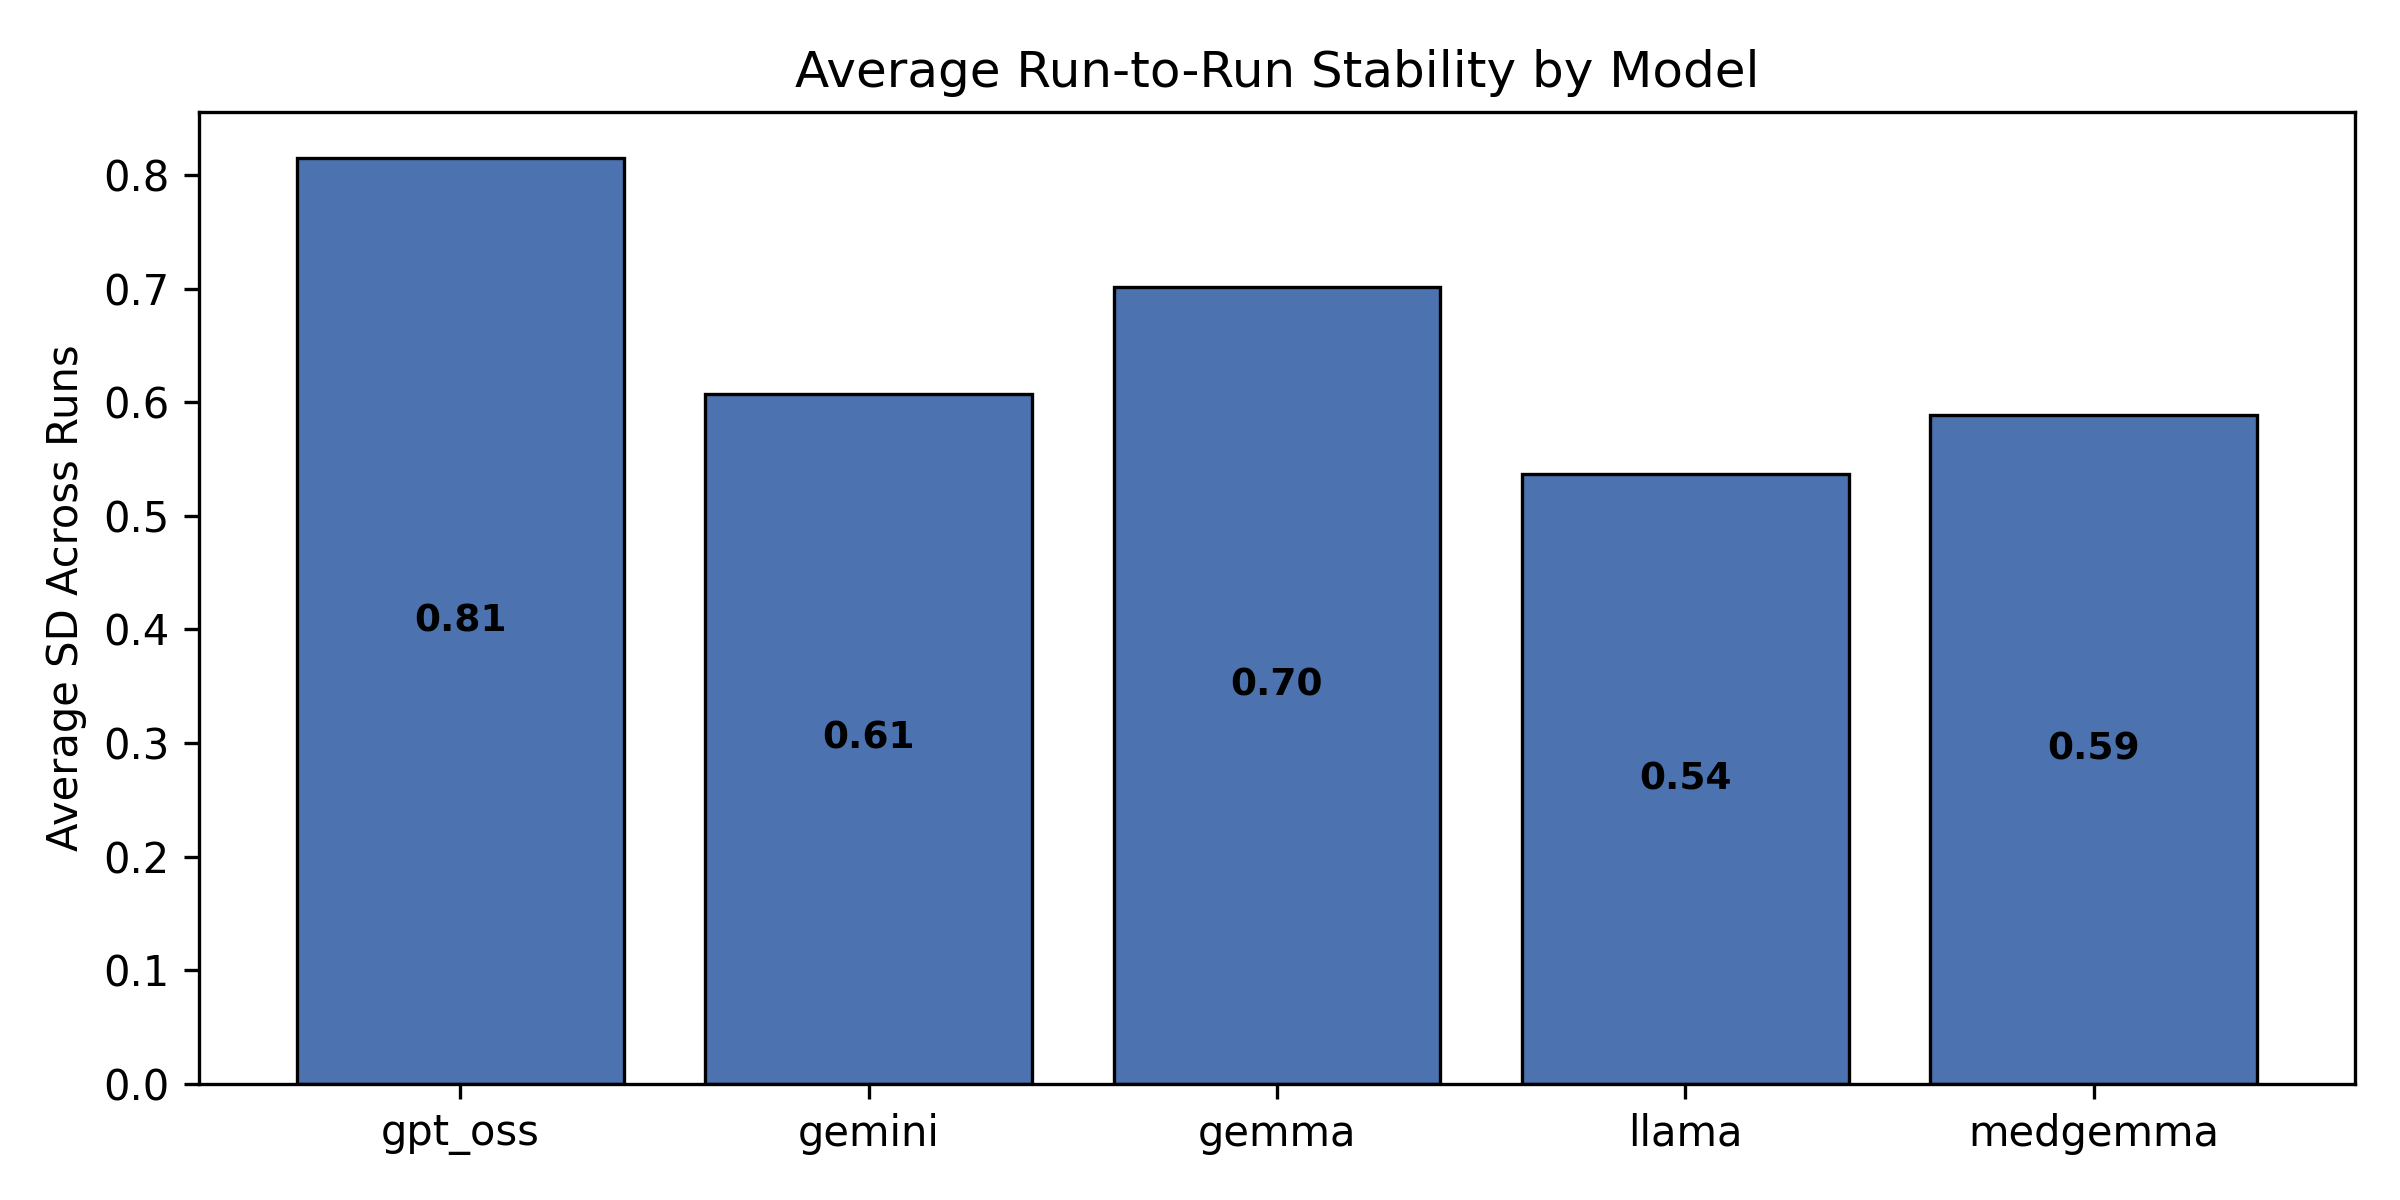
\includegraphics[width=\columnwidth]{Q3_STABILITY.png}
    \caption{\textbf{Run-to-run stability across models.} Bars show the average standard deviation (SD) of diagnostic scores across three independent runs per vignette. Higher values indicate greater output variability. \texttt{GPT-OSS} exhibits the highest stochasticity (SD = 0.81), while \texttt{LLaMA} (SD = 0.54) and \texttt{MedGemma} (SD = 0.59) demonstrate the greatest consistency.}
    \label{fig:stability}
\end{figure}

\subsection{Rubric Components Show Task-Specific Micro-Variation}

Component-level analysis revealed that training background effects remain non-significant even when examined at finer granularity (Table~\ref{tab:rubric}, Figure~\ref{fig:heatmap_sensitivity}). An isolated uncorrected effect appeared in Gemini-2.5's Diagnosis List component (Pakistani $\Delta = -0.101$, $p = 0.040$), but failed FDR correction ($p_{\text{FDR}} = 0.200$).

In contrast, operational constraints produced consistent directional effects. Limited resources disproportionately impacted Final Diagnosis ($q4$) and Additional Steps ($q5$), while step-by-step reasoning improved Supporting Evidence ($q2$) and Opposing Evidence ($q3$). These patterns suggest that models adapt diagnostic reasoning to stated constraints but do not spontaneously infer resource limitations from identity labels alone.

Heatmap visualization confirms absence of systematic column-wide underperformance for the Pakistani persona. Observed differences reflect task-specific model behaviors rather than identity-driven bias.

\begin{table}[htbp]
\centering
\caption{Directional effects of persona dimensions on rubric components. Arrows indicate consistent trends; ``ns'' denotes non-significant effects after FDR correction.}
\label{tab:rubric}
\begin{tabular}{|l|c|c|c|}
\hline
\textbf{Rubric} &
\textbf{Training} &
\textbf{Resources} &
\textbf{Step-by-step} \\
\textbf{Component} &
\textbf{(Pak vs US)} &
\textbf{(Limited)} &
\textbf{(Yes)} \\
\hline
Diagnosis list      & ns & $\downarrow$ & $\uparrow$ \\
Supporting evidence & ns & $\downarrow$ & $\uparrow^{*}$ \\
Opposing evidence   & ns & $\downarrow$ & $\uparrow$ \\
Final diagnosis     & ns & $\downarrow^{*}$ & $\uparrow$ \\
Additional steps    & ns & $\downarrow$ & $\uparrow$ \\
\hline
\end{tabular}

\vspace{0.5em}
\footnotesize{$^{*}$ Model-specific effect (MedGemma).}
\end{table}

\begin{figure}[t]
    \centering
    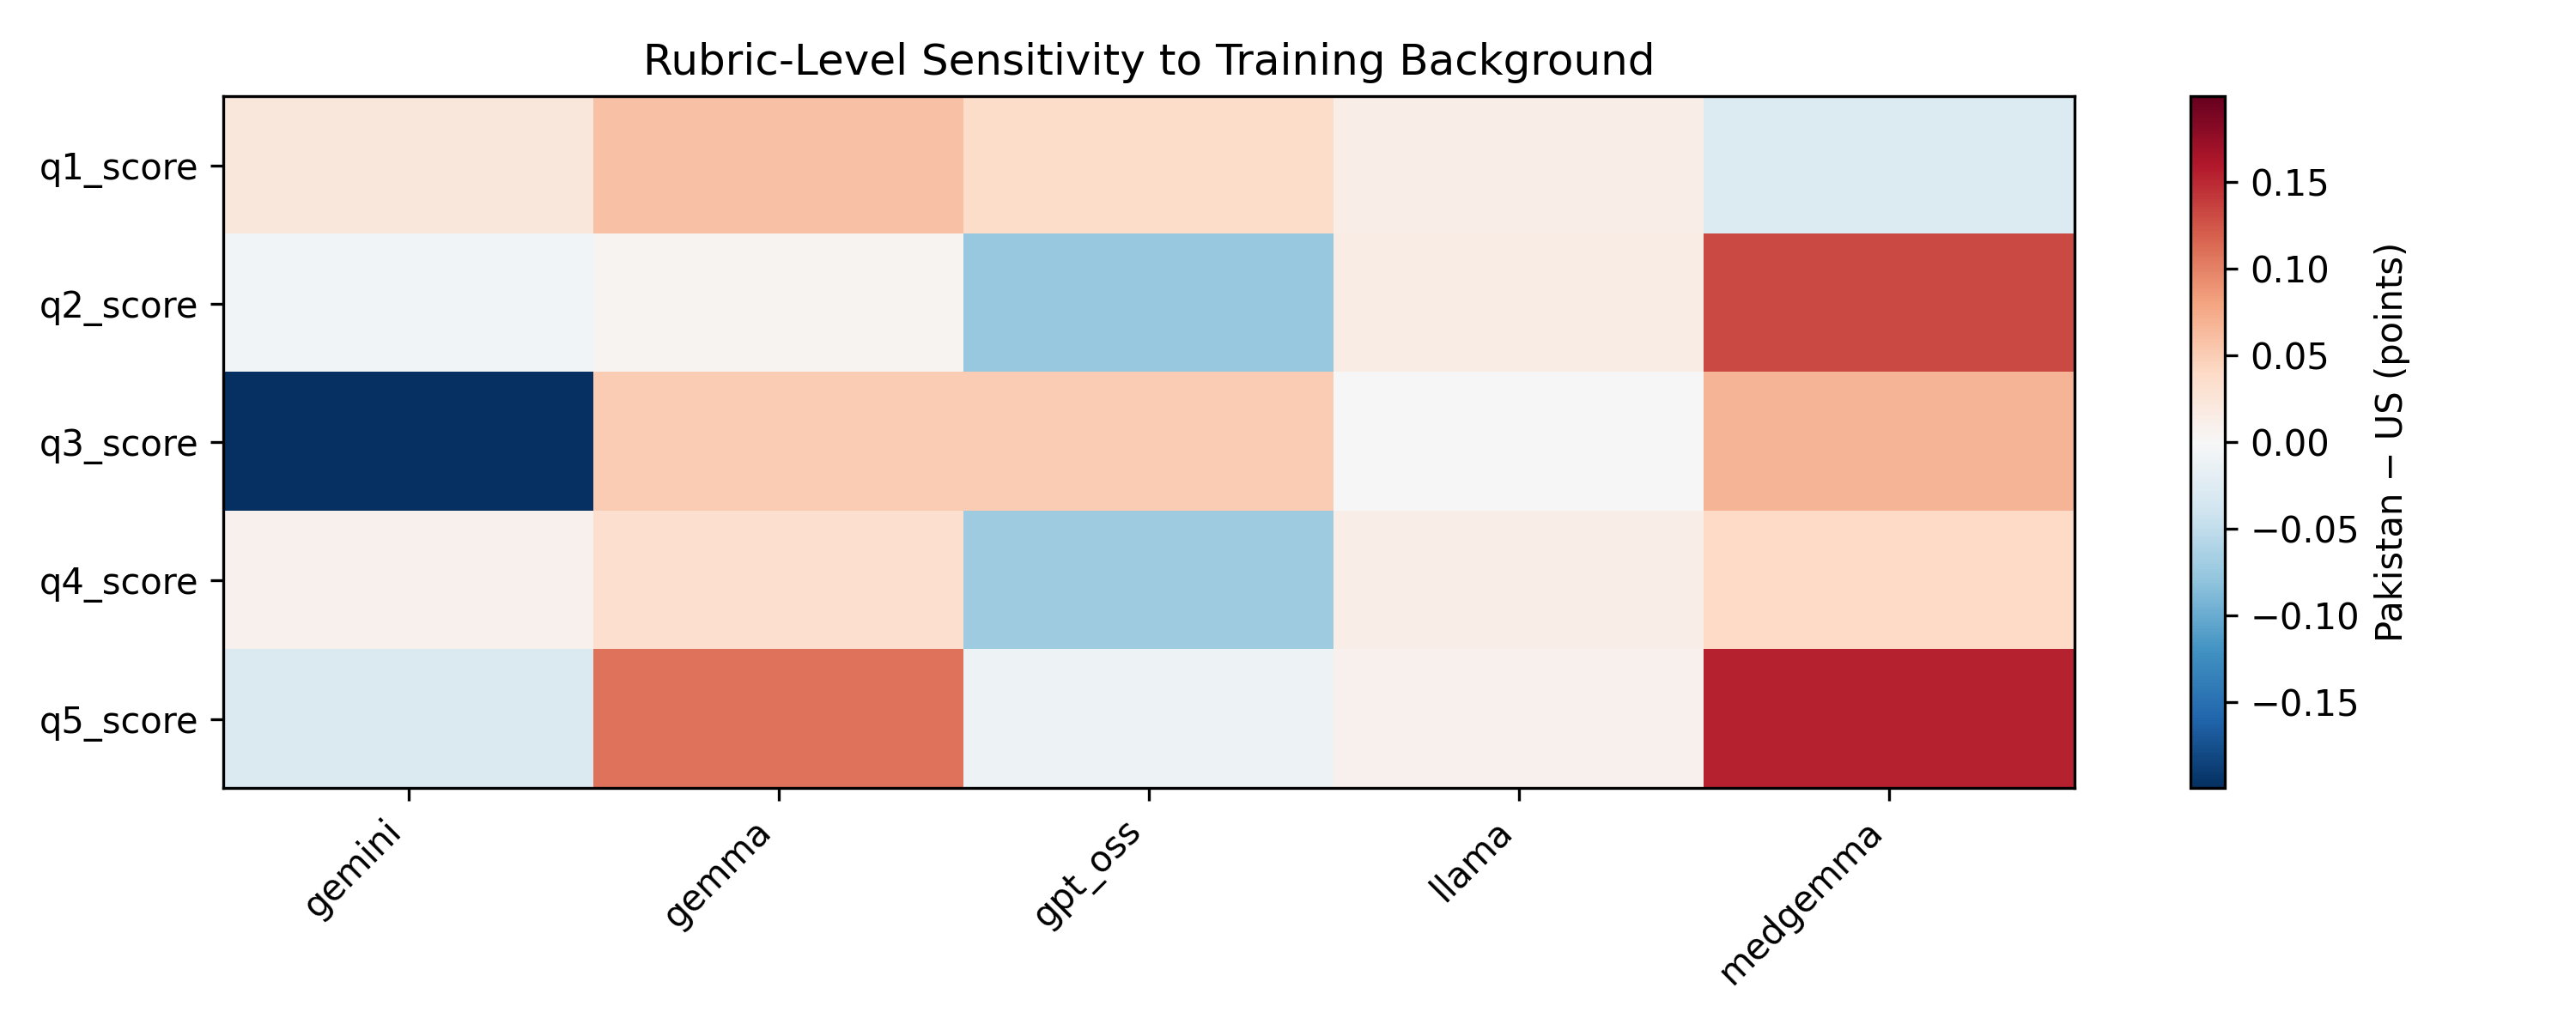
\includegraphics[width=\columnwidth]{HEATMAP_SENSTIVITY.png}
    \caption{\textbf{Rubric-level sensitivity to simulated training background.} Heatmap shows the mean score difference between Pakistani and US personas (Pakistan -- US) for each rubric component and model. Red indicates higher performance for the Pakistani persona, blue indicates lower performance. Differences are small in magnitude ($|\Delta| \leq 0.15$) and vary by task and model rather than exhibiting a uniform directional pattern.}
    \label{fig:heatmap_sensitivity}
\end{figure}


\section{Discussion}

\subsection{The Hollow Persona Phenomenon: Identity Labels Without Knowledge Shift}

The central finding of this study is that contemporary LLMs exhibit training background neutrality: simulated national-origin personas do not meaningfully alter diagnostic performance. This pattern held across five architectures, 13 clinical vignettes, and 5,070 observations, with effect sizes consistently smaller than measurement noise.

We conceptualize this as a "Hollow Persona" effect.The Hollow Persona phenomenon refers specifically to identity-based persona labels provided without explicit operational context. It does not suggest that personas are inherently ineffective, but rather that identity cues alone are insufficient to induce meaningful shifts in clinical knowledge retrieval or reasoning strategies in current LLMs.

While LLMs can superficially adopt the rhetorical framing of a Pakistani- or US-trained physician, they do not fundamentally shift their knowledge retrieval strategies. The Pakistani persona does not spontaneously prioritize dengue over Lyme disease, nor does it recognize that MRI availability is limited without explicit instruction. Instead, both personas draw from the same knowledge distribution—one heavily weighted toward high-resource, Western medical literature. This example is illustrative rather than exhaustive and highlights the absence of systematic regional prioritization, not isolated instances of correct disease mention.

This finding contradicts the hypothesis that identity-based prompting would trigger performance degradation in LMIC contexts. However, it also reveals a critical limitation: LLMs fail to simulate authentic regional medical reasoning because such reasoning patterns are underrepresented in training data. The absence of bias does not imply cultural competence; it reflects homogenization.

The implications are twofold. First, explicit concerns about identity-triggered bias in diagnostic accuracy appear unfounded for current models. Second, achieving genuine equity requires moving beyond surface-level persona labels toward operational grounding—explicitly specifying epidemiology, resource constraints, and local guidelines.

These findings should be interpreted within the scope of diagnostic vignette-based reasoning tasks and do not necessarily extend to downstream clinical decision-making, patient interaction, or longitudinal care scenarios.

\subsection{Operational Prompting as the True Lever for Global Health AI}

If identity is a weak signal, what drives performance? Our results demonstrate that operational constraints—explicitly defined resource availability, reasoning scaffolds, and task framing—produce effects approximately 4–6 times larger than any identity-based persona dimension, as measured by changes in total diagnostic score.

The most pronounced effect was resource limitation. Explicitly stating that advanced diagnostics were unavailable reduced scores by 1.55 points, primarily in the Final Diagnosis and Additional Steps components. This reduction should not be interpreted as model failure or degraded clinical reasoning. Instead, it reflects appropriate context-sensitive adaptation: models constrained diagnostic recommendations when informed that confirmatory tests were inaccessible. Importantly, this score reduction arises from a misalignment between the evaluation rubric and context-aware reasoning rather than a decline in diagnostic logic. The rubric implicitly rewards comprehensive diagnostic exploration characteristic of high-resource settings, whereas the models adjusted recommendations in response to stated resource constraints.

This finding has direct implications for global health deployment. Many evaluation frameworks implicitly assume universal access to advanced diagnostics. When models are deployed in resource-constrained settings without explicit operational prompting, they may recommend infeasible tests, reducing practical usefulness. Conversely, when constraints are specified, models adapt appropriately, but existing rubrics may fail to reward this behavior as clinically reasonable reasoning.

Step-by-step reasoning prompts consistently improved performance, particularly in evidence synthesis components. This effect was strongest for MedGemma, suggesting that medically fine-tuned models benefit disproportionately from cognitive scaffolding. In contrast, guideline-based prompts paradoxically reduced performance, likely because the evaluation rubric favors expansive differential generation while clinical guidelines emphasize diagnostic parsimony. This tension highlights a broader challenge for clinical LLM evaluation: scoring frameworks must align with the intended clinical objective of the prompt.


\subsection{Model-Specific Profiles and Deployment Considerations}

Analysis revealed distinct behavioral signatures with implications for real-world deployment:

\paragraph{MedGemma: The Stable Specialist} 
Demonstrated the highest run-to-run consistency ($r > 0.7$) and greatest responsiveness to step-by-step prompting, suggesting reliability for structured clinical protocols. However, lower absolute performance indicates need for ensemble methods or human oversight.

\paragraph{LLaMA-3.1: The Context-Aware Generalist}
Uniquely sensitive to socioeconomic context ($\Delta = 0.93$, $p = 0.013$), suggesting strength in public health applications where social determinants matter. High stability ($r \approx 0.66$) supports use in low-stakes monitoring scenarios.

\paragraph{GPT-OSS: The Volatile High-Performer}
Achieved near-Gemini accuracy but with concerning instability ($r \approx 0.3$). Identical prompts yielded divergent outputs, indicating unsuitability for autonomous decision-making without self-consistency sampling or ensemble averaging.

\paragraph{Gemini-2.5: The Balanced Benchmark}
Combined highest absolute accuracy with moderate consistency, representing the current state-of-the-art for clinical LLM deployment. However, even this model exhibited no sensitivity to identity labels, confirming that architectural sophistication does not confer cultural competence.


\subsection{Implications for Fairness Evaluation and Global Health AI}

These findings challenge prevailing assumptions in medical AI fairness research. Much existing work evaluates models for demographic bias by comparing outputs across identity groups. Our results suggest this approach may be insufficient: absence of explicit bias (training background neutrality) does not guarantee equitable utility across contexts.From an evaluation perspective, this implies that fairness assessments should move beyond identity-based comparisons and explicitly test whether models adapt appropriately to changes in clinical context, resources, and epidemiology under controlled conditions.

The Hollow Persona phenomenon reveals that fairness is not solely about preventing harm—it is also about enabling appropriate, context-aware reasoning. A model that treats all personas identically may still produce inequitable outcomes if its knowledge base lacks regional epidemiology, local treatment guidelines, or resource-appropriate diagnostic pathways.

Future fairness frameworks must therefore assess not only \emph{differential treatment} but also \emph{contextual appropriateness}. Evaluation should test whether models correctly adapt reasoning when epidemiological base rates differ, when standard-of-care diagnostics are unavailable, or when clinical guidelines diverge. Our findings suggest that current models require explicit operational prompting to achieve this adaptation—they do not infer it from clinician identity alone.

For global health deployment, this implies a shift from identity-aware prompting to \emph{context-aware engineering}. Rather than instructing a model "You are a doctor in Pakistan," practitioners should specify "Dengue is endemic; MRI unavailable; follow WHO guidelines for resource-limited settings." This operational grounding enables models to retrieve relevant knowledge and adapt reasoning appropriately.


\section{Limitations and Future Directions:}
This study relies on a single judge model (Llama 3.3) and a finite set of 13 clinical vignettes, which may constrain the generalizability of our absolute performance metrics. While the use of a single judge ensures high internal consistency for comparative analysis, avoiding the inter-rater noise inherent in multi-judge systems (Seo et al., 2025), it leaves open the possibility that the judge model itself possesses blind spots regarding specific medical guidelines. Furthermore, while our vignettes were verified by a panel of five physicians to ensure complexity and accuracy, they remain text-based simplifications of real-world patient encounters.
Future work should aim to validate these findings using a "human-in-the-loop" approach, where a subset of cases is adjudicated by human clinicians to calibrate the automated rubric scores. Additionally, expanding the vignette library to include "trap" cases, specifically designed where US and Pakistani guidelines diverge, would provide a more stress-tested evaluation of the "Hollow Persona" hypothesis. Nonetheless, the remarkable consistency of our null findings across five distinct model architectures and thousands of observations supports the robustness of the conclusion: simulated identity is a weak lever for performance compared to operational constraints.


\section{Conclusion}
In summary, fears of hidden geographic bias encoded in LLM personas may be overstated when tasks are purely diagnostic. Across five leading models, we found that diagnostic equity is less a matter of who the model pretends to be (Identity) and more a matter of how the clinical environment is specified (Context).
We observe a "Hollow Persona" phenomenon where national identity labels act as superficial stylistic modifiers rather than keys to distinct knowledge distributions. A "Pakistani-trained" persona does not inherently degrade performance; however, it also does not automatically summon local epidemiological knowledge unless explicitly prompted. Therefore, advancing global health AI will require rigorous operational grounding, explicitly defining resource constraints (e.g., "No MRI access"), enforcing structured reasoning (e.g., "Step-by-step"), and verifying stability, rather than relying on vague identity prompts to do the heavy lifting. Equitable deployment is an engineering challenge of specification, not just a representational challenge of identity.

\newpage
\section{References}

Suenghataiphorn, T.; Tribuddharat, N.; Danpanichkul, P.; and Kulthamrongsri, N. 2025.
Bias in Large Language Models Across Clinical Applications: A Systematic Review.
arXiv preprint arXiv:2504.02917.

Omar, M.; Sorin, V.; Agbareia, R.; Apakama, D. U.; Soroush, A.; Sakhuja, A.;
Freeman, R.; Horowitz, C. R.; Richardson, L. D.; Nadkarni, G. N.; and Klang, E.
2025. Evaluating and addressing demographic disparities in medical large language
models: A systematic review. \textit{International Journal for Equity in Health},
24(1): 57.

Zhou, Y.; Di Eugenio, B.; and Cheng, L. 2025.
Unveiling Performance Challenges of Large Language Models in Low-Resource Healthcare:
A Demographic Fairness Perspective. In \textit{Proceedings of the 2025 Conference on
Computational Linguistics (COLING)}.

Nature Editorial Team. 2025.
Large Language Models in Biomedicine and Healthcare.
\textit{npj Artificial Intelligence}, 1: 47.

Smith, J.; Bai, N.; Yu, Y.; Luo, C.; Zhou, S. C.; Wang, Q.; Zou, H.; Liu, Q.;
Fu, G.; Zhai, W.; Zhao, Q.; Li, J.; Wei, X.; and Yang, B. X. 2025.
Detecting Sociodemographic Biases in the Content and Quality of Large Language
Model-Generated Nursing Care: Cross-Sectional Simulation Study.
\textit{Journal of Medical Internet Research}, 27: e78132.

Suenghataiphorn, K.; Rahman, M.; Banerjee, I.; and Patel, V. 2025.
Bias and Fairness in Clinical Large Language Models: A Systematic Review.
\textit{arXiv preprint} arXiv:2504.02917.

Omar, R.; El-Shahawy, M.; and Bender, E. 2025.
Demographic Biases in Medical Large Language Models: A Systematic Review.
\textit{International Journal for Equity in Health}, 24(1): Article 19.

Zhou, Y.; Lin, J.; and Wang, X. 2025.
Evaluating Fairness After Instruction Tuning in Large Language Models.
\textit{AI}, 6(5): 106.

Hida, K.; Tanaka, S.; and Okazaki, N. 2025.
Prompt Sensitivity and Bias Variability in Large Language Models.
In \textit{Findings of the 2025 Conference on Empirical Methods in Natural Language Processing (EMNLP Findings)}.
Association for Computational Linguistics.

Patel, R.; Desai, A.; and Kumar, S. 2025.
Assessing Sociodemographic Bias in AI-Generated Nursing Care Plans.
\textit{JMIR Public Health and Surveillance}, 11(1): e78132.

Reuters. 2025.
Health Rounds: AI Can Have Medical Care Biases Too, Study Reveals.
Reuters News, April 9, 2025.

Smith, J.; Alvarez, M.; and Chen, L. 2025.
Bias in Clinical Large Language Models for LGBTQIA+ Health Scenarios.
\textit{Journal of Medical Ethics}, 51(4): 245--252.

Wang, T.; Ho, D.; and Koyejo, S. 2025.
Performance Degradation in Personalized Large Language Models.
In \textit{Proceedings of the AAAI Conference on Artificial Intelligence (AAAI 2025)}.

Lee, S.; Su, H.; Sun, Y.; Li, R.; Zhang, A.; Yang, Y.; Xiao, F.; Duan, Z.;
Chen, J.; Hu, Q.; Yang, T.; Xu, B.; Zhang, Q.; Zhao, J.; Li, Y.; and Li, H. 2025.
Large Language Models in Medical Diagnostics: Scoping Review with Bibliometric Analysis.
\textit{Journal of Medical Internet Research}, 27: e72062.

Lin, S.; Hilton, J.; and Evans, O. 2022.
TruthfulQA: Measuring How Models Mimic Human Falsehoods.
In \textit{Proceedings of the 60th Annual Meeting of the Association for Computational Linguistics (ACL)}.

Perez, E.; Ribeiro, M. T.; Singh, S.; and Guestrin, C. 2023.
Discovering Language Model Behaviors with Model-Written Evaluations.
In \textit{Proceedings of the 2023 Conference on Neural Information Processing Systems (NeurIPS)}.

Laban, P.; Hsu, W.-N.; and Hearst, M. 2023.
When Do Language Models Admit Their Mistakes?
In \textit{Findings of the Association for Computational Linguistics (ACL Findings)}.

Ranaldi, L.; and Pucci, G. 2023.
Preferential Agreement Bias in Large Language Models.
In \textit{Proceedings of the 2023 Conference on Empirical Methods in Natural Language Processing (EMNLP)}.

Sharma, A.; Durmus, E.; and Wallace, B. 2024.
Political Bias and Sycophancy in Large Language Models.
In \textit{Proceedings of the 2024 Conference of the North American Chapter of the Association for Computational Linguistics (NAACL)}.

Abid, A.; Farooqi, M.; and Zou, J. 2021.
Persistent anti-Muslim bias in large language models.
In \textit{Proceedings of the 2021 AAAI/ACM Conference on AI, Ethics, and Society}, 298--306.

Bates, D.; M{\"a}chler, M.; Bolker, B.; and Walker, S. 2015.
Fitting linear mixed-effects models using lme4.
\textit{Journal of Statistical Software}, 67(1):1--48.

Benjamini, Y.; and Hochberg, Y. 1995.
Controlling the false discovery rate: a practical and powerful approach to multiple testing.
\textit{Journal of the Royal Statistical Society: Series B (Methodological)}, 57(1):289--300.

Chang, Y.; Wang, X.; Wang, J.; Wu, Y.; Yang, L.; Zhu, K.; Chen, H.; Yi, X.; Wang, C.; Wang, Y.; and others. 2023.
A survey on evaluation of large language models.
\textit{ACM Transactions on Intelligent Systems and Technology}, 15(3):1--45.

Deshpande, A.; Murahari, V.; Rajpurohit, T.; Kalyan, A.; and Narasimhan, K. 2023.
Persona-based evaluation of language models.
In \textit{Proceedings of the 2023 Conference on Empirical Methods in Natural Language Processing}, 3856--3879.

Gichoya, J. W.; McCoy, L. G.; Celi, L. A.; and Ghassemi, M. 2021.
AI in global health: The need for an equitable framework.
\textit{The Lancet Digital Health}, 3(9):e539--e541.

Jin, Q.; Chen, F.; Zhou, Y.; Mao, Z.; Liu, J.; Yu, D.; Franzen, D.; Liang, J.; Lu, X.; and others. 2023.
Evaluating large language models on medical evidence summarization.
\textit{npj Digital Medicine}, 6(1):158.

Kelly, C. J.; Karthikesalingam, A.; Suleyman, M.; Corrado, G.; and King, D. 2023.
Key challenges for evaluating clinical AI systems.
\textit{The Lancet Digital Health}, 5(4):e222--e223.


Obermeyer, Z.; Powers, B.; Vogeli, C.; and Mullainathan, S. 2019.
Dissecting racial bias in an algorithm used to manage the health of populations.
\textit{Science}, 366(6464):447--453.

Rajpurkar, P.; Chen, E.; Banerjee, O.; and Topol, E. J. 2022.
AI in health and medicine.
\textit{Nature Medicine}, 28(1):31--38.

Siala, M. A.; and Wang, Y. 2024.
AI for global health equity: Opportunities and challenges in low-resource settings.
\textit{Journal of Global Health}, 14:03001.

Singhal, K.; Azizi, S.; Tu, T.; Mahdavi, S. S.; Wei, J.; Chung, H. W.; Scales, N.; Tanwani, A.; Cole-Lewis, H.; Pfohl, S.; and others. 2023.
Large language models encode clinical knowledge.
\textit{Nature}, 620(7972):172--180.

Weng, Y.; Xu, R.; Wu, Y.; Li, W.; Wang, J.; Chen, Y.; Zhang, Y.; Zhu, Z.; Ye, J.; Chen, H.; and others. 2023.
Systematic review of fairness in artificial intelligence algorithms for medical imaging.
\textit{Medical Image Analysis}, 89:102911.

Whitaker, K.; Price, W. N.; and Cohen, I. G. 2023.
Fairness in machine learning for health care.
\textit{Annual Review of Biomedical Data Science}, 6:195--217.
\end{document}
